% FEP-RLVE — NeurIPS-format mini-paper.
% Requires the official NeurIPS style file `neurips_2024.sty` in this directory
% (download from https://neurips.cc/Conferences/2024/PaperInformation/StyleFiles,
%  or open the "NeurIPS 2024" template on Overleaf and drop main.tex/refs.bib in).
% Build:  pdflatex main ; bibtex main ; pdflatex main ; pdflatex main
\documentclass{article}

\usepackage[final]{neurips_2024}

\usepackage[utf8]{inputenc}
\usepackage[T1]{fontenc}
\usepackage{hyperref}
\usepackage{url}
\usepackage{booktabs}
\usepackage{amsfonts}
\usepackage{amsmath}
\usepackage{amssymb}
\usepackage{graphicx}
\usepackage{xcolor}
\usepackage{enumitem}

\newcommand{\UK}{U_{K}}
\newcommand{\Eq}[1]{\mathbb{E}_{q}\!\left[#1\right]}
\newcommand{\KL}{D_{\mathrm{KL}}}

\title{FEP-RLVE: Difficulty Selection as Active Inference for Reinforcement Learning on Verifiable Environments}

\author{%
  Lian Cheng \quad Yu Bao \quad Licheng Wen \\
  Shanghai Innovation Institute \\
  \texttt{\{chenglian\}@baoyu.space}
}

\begin{document}

\maketitle

\begin{abstract}
Reinforcement learning (RL) post-training of reasoning LLMs stalls when task
difficulty drifts off the model's capability frontier: under group-relative
objectives (GRPO/DAPO) a group of $K$ rollouts that is all-correct or all-wrong
has zero advantage variance and yields \emph{no} gradient. RL with verifiable
environments (RLVE) keeps problems solvable through procedurally generated,
algorithmically verified tasks with adaptive difficulty, but raises difficulty
only once accuracy exceeds a threshold ($\tau_{\mathrm{acc}}{=}0.9$)---a
one-directional heuristic that parks the model in a low-signal regime
($\UK(0.9){=}0.34 \ll \UK(0.5){=}0.875$ at $K{=}4$). We recast difficulty
selection as \textbf{active inference}: the trainer maintains a belief
$q(s_e)$ over each environment's latent competence, updates it by minimizing
\emph{variational} free energy (a Bayesian belief update; perception), and
selects the next difficulty by minimizing \emph{expected} free energy
$G_e(d) = \lambda_{\mathrm{sig}}\,(-\ln \UK(\hat p(d))) - \lambda_{\mathrm{info}}\,I(s_e;o\mid d) + \lambda_{\mathrm{cost}}\,C(d)$,
sampling $\pi(d)\propto\exp(-G_e(d)/T)$. The pragmatic term is a preference
\emph{risk} that is minimal at the signal-optimal $p{=}0.5$ band and diverges at
degenerate difficulties; the epistemic term actively probes competence and moves
difficulty in \emph{both} directions. RLVE is the degenerate case
$\lambda_{\mathrm{info}}{=}0,\ T{\to}0$ with a high-accuracy preference. We
implement the controller as a drop-in replacement for RLVE's scheduler and run a
controlled 3-arm comparison (RLVE-90, a pragmatic-only ablation Signal-RLVE, and
full FEP-RLVE) reproduced from ProRL-1.5B-v2 on a single H200. At this scale the
controllers regulate difficulty as designed---FEP-RLVE holds steady-state success
closest to the informative $0.5$ set-point---while held-out generalization does
\emph{not} separate the arms. A mechanistic analysis attributes this to severe
response truncation that makes rollout groups degenerate, so the \emph{realized}
gradient is far below the \emph{expected} $\UK$; we report this gap as the
binding constraint rather than overclaiming a generalization win.
\end{abstract}

\section{Introduction}
RL post-training of reasoning models needs a \emph{sustained} supply of
mid-difficulty experience. If problems are too hard the verifier almost always
returns failure (reward sparsity); if too easy the model already solves them and
the signal decays. Under group-relative policy optimization
(GRPO~\citep{shao2024deepseekmath}, DAPO~\citep{yu2025dapo}) this is sharp: the
advantage of a rollout is its reward centered and scaled \emph{within its group}
of $K$ samples, so a group that is unanimously correct or unanimously wrong has
zero variance and contributes exactly zero gradient---DAPO discards such groups
outright. The trainable signal therefore lives in \emph{informative} groups with
$0 < \sum_k o_k < K$.

RL with verifiable environments (RLVE)~\citep{zeng2025rlve} keeps problems in this
band by generating tasks from procedural environments with algorithmic verifiers
and a scalar difficulty knob, and by scaling the \emph{number} of environments to
improve generalization~\citep{scaler2026}. Its difficulty controller, however, is
a one-directional heuristic: per environment, raise the difficulty ceiling once
the success rate at the ceiling exceeds $\tau_{\mathrm{acc}}{=}0.9$. This parks
the model at high accuracy---precisely a \emph{low-signal} regime---never lowers
difficulty if the model regresses, and has no explicit objective or exploration.

We make three contributions.
\begin{enumerate}[leftmargin=1.4em,itemsep=1pt,topsep=1pt]
\item We show RLVE's $0.9$ threshold is signal-suboptimal: the probability that a
$K$-group is informative is $\UK(p)=1-p^K-(1-p)^K$, uniquely maximized at
$p=0.5$, so the gradient supply collapses as the controller pushes $p\!\to\!1$
(\S\ref{sec:method}, App.~A).
\item We recast difficulty selection as \textbf{active inference} (Friston's Free
Energy Principle~\citep{friston2010free,dacosta2020active}): a generative model of
latent competence, a variational-free-energy belief update (perception), and an
\textbf{expected free energy} objective whose pragmatic term is the preference
risk $-\ln \UK$ and whose epistemic term is the information gain about competence
(\S\ref{sec:method}, App.~B). RLVE is recovered as a degenerate special case.
\item We provide a dependency-free controller dropped into RLVE's scheduler and a
controlled same-compute comparison that isolates the epistemic term
(RLVE-90 / Signal-RLVE / FEP-RLVE), reported with an honest mechanistic analysis
of why the arms do not separate on held-out at this scale
(\S\ref{sec:setup}--\S\ref{sec:discussion}).
\end{enumerate}

\section{Background}
\textbf{Verifiable environments.} An RLVE environment is a procedural generator
plus an algorithmic verifier exposing a scalar difficulty $d$; a sample at
difficulty $d$ yields a binary correctness outcome $o\in\{0,1\}$. \textbf{GRPO/DAPO}
draw $K$ rollouts per prompt and use the group-centered reward as the advantage,
so zero-variance groups carry no gradient (App.~A.1). \textbf{RLVE's controller}
tracks accuracy at the difficulty ceiling and bumps it when $\mathrm{acc}\ge 0.9$;
it is one-directional and threshold-based. \textbf{Active inference}~\citep{friston2010free,dacosta2020active}
splits an agent's free-energy minimization into \emph{perception} (update beliefs
about hidden states by minimizing variational free energy $=$ Bayesian inference)
and \emph{action} (choose policies that minimize \emph{expected} free energy, a
sum of a pragmatic preference term and an epistemic information-gain term).

\section{Method: Difficulty Selection as Active Inference}
\label{sec:method}

\subsection{Learning utility: the signal peaks at \texorpdfstring{$p=0.5$}{p=0.5}}
For binary correctness with per-group success probability $p$, a group of $K$
i.i.d.\ rollouts is informative iff $0<\sum_k o_k<K$, with probability
\begin{equation}
\UK(p) \;=\; 1 - p^K - (1-p)^K,
\end{equation}
uniquely maximized at $p^\star=0.5$ for all $K\ge 2$ (App.~A.2), where it also
maximizes the expected within-group reward variance that scales the advantages
(App.~A.3). Figure~\ref{fig:uk} shows the curve: at $K{=}4$, $\UK(0.5)=0.875$
whereas $\UK(0.9)=0.34$. Because success $p(d)$ decreases monotonically in
difficulty $d$, there is a difficulty $d^\star$ with $p(d^\star)=0.5$ that
maximizes the expected learning signal; RLVE's rule instead targets $p\approx0.9$.

\begin{figure}[t]
\centering
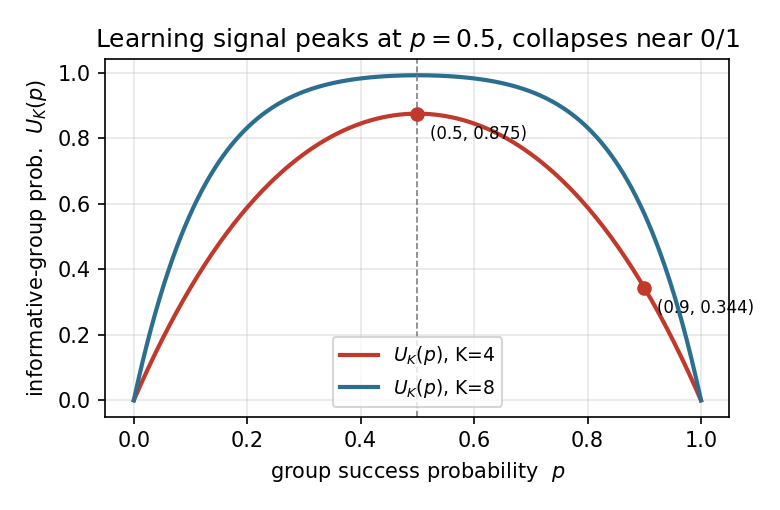
\includegraphics[width=0.52\linewidth]{figures/uk_curve.png}
\caption{Informative-group probability $\UK(p)=1-p^K-(1-p)^K$. The learning
signal is maximal at $p=0.5$ and collapses as $p\!\to\!0$ or $1$. RLVE's
$\mathrm{acc}\ge0.9$ operating point ($\UK{=}0.34$ at $K{=}4$) is far down the
right shoulder.}
\label{fig:uk}
\end{figure}

\subsection{Perception: a generative model of competence and its belief update}
For environment $e$, let $s_e\in\mathbb{R}$ be the model's latent \textbf{competence}.
Following item-response theory~\citep{rasch1960probabilistic}, the outcome at
difficulty $d$ is generated by
\begin{equation}
P(o=1\mid s_e,d) \;=\; \sigma\!\big(a\,(s_e-d)\big),
\end{equation}
with discrimination $a$. The trainer maintains a belief $q(s_e)$ (a grid over
$s_e$); predicted success is $\hat p(d)=\mathbb{E}_{s\sim q}[\sigma(a(s-d))]$.
Given a batch of outcomes, the \emph{variational free energy}
\begin{equation}
F[q]=\Eq{\ln q(s)-\ln p(o,s)}=\KL\!\big(q(s)\,\|\,p(s\mid o)\big)-\ln p(o)
\end{equation}
is minimized by the Bayesian posterior, i.e.\ the exact grid update
$q(s)\leftarrow q(s)\prod_k P(o_k\mid s,d_k)/Z$ (perception; App.~B.2). The belief
is maintained \emph{per environment} and updated only from that environment's
own outcomes.

\subsection{Action: expected free energy over difficulties}
To choose the next difficulty, active inference minimizes the expected free energy
\begin{equation}
G_e(d) \;=\; \underbrace{\lambda_{\mathrm{sig}}\,\big(-\ln \UK(\hat p(d))\big)}_{\text{pragmatic / preference risk}}
\;-\; \underbrace{\lambda_{\mathrm{info}}\,I_q(s_e;o\mid d)}_{\text{epistemic / info gain}}
\;+\; \lambda_{\mathrm{cost}}\,C(e,d).
\label{eq:efe}
\end{equation}
The preference is over \emph{outcomes}, and crucially is not ``always correct''
(which would prefer easy tasks) but ``the group is \emph{informative}'', whose
predicted probability is $\UK(\hat p(d))$; the preference risk
$\mathbb{E}_{q(o\mid d)}[-\ln P_{\mathrm{pref}}(o)]=-\ln \UK(\hat p(d))$ is minimal
at $p{=}0.5$ and diverges as $\UK\!\to\!0$, strongly repelling degenerate
(all-pass/all-fail) difficulties (App.~B.3). The epistemic term is the mutual
information $I_q(s_e;o\mid d)=H[\mathrm{Ber}(\hat p)]-\mathbb{E}_{s\sim q}H[\mathrm{Ber}(\sigma(a(s-d)))]$,
largest where outcomes are most diagnostic of competence; its location tracks the
current belief uncertainty rather than a fixed $0.5$ target, letting the
controller actively probe the frontier. The policy is the active-inference softmax
\begin{equation}
\pi(d\mid e)\;\propto\;\exp\!\big(-G_e(d)/T\big),
\end{equation}
greedy as $T\!\to\!0$ and uniform as $T\!\to\!\infty$. \textbf{RLVE is the
degenerate case} $\lambda_{\mathrm{info}}{=}0$, $T\!\to\!0$, with a high-accuracy
(rather than informative-band) preference (App.~B.5). Setting only
$\lambda_{\mathrm{info}}{=}0$ gives our \emph{Signal-RLVE} ablation, which targets
$p{=}0.5$ but does not probe competence.

\subsection{Online controller}
The belief is a per-environment grid (exact Bayes; no Gaussian/Laplace
approximation); \texttt{observe()} performs the update, \texttt{G()}/\texttt{policy()}
score and sample difficulties. The controller is dependency-free and self-checked
($\UK$ and information gain both peak at $p{=}0.5$; belief $\sigma$ contracts as
competence rises). It is wired into RLVE's SLIME rollout scheduler, replacing the
$\mathrm{acc}\ge0.9$ bump and leaving the RL core (GRPO) unchanged.

\section{Experimental setup}
\label{sec:setup}
We reproduce RLVE on the SLIME backend from \textbf{ProRL-1.5B-v2}
(\texttt{Nemotron-Research-Reasoning-Qwen-1.5B})~\citep{liu2025prorl} on a single
H200 (the official 8-GPU recipe reconfigured to one card; see
\texttt{rlve\_repro/}). Training uses $4$ environments for $30$ rollout steps with
$K{=}4$ samples per prompt (rollout batch $8$, oversample $8$), difficulty range
$[0,16]$, controller temperature $T{=}0.25$, $\lambda_{\mathrm{sig}}{=}1$,
$\lambda_{\mathrm{cost}}{=}0$, response budget $2048$ tokens. We evaluate on a
fixed held-out set of $128$ environment instances at steps $0,9,19,29$. Three arms
share the \emph{same} recipe and differ \emph{only} in the difficulty controller:
\textbf{RLVE-90} (the $\mathrm{acc}\ge0.9$ baseline), \textbf{Signal-RLVE}
($\lambda_{\mathrm{info}}{=}0$), and \textbf{FEP-RLVE} ($\lambda_{\mathrm{info}}{=}1$).
Signal-RLVE is the key ablation: only if FEP-RLVE beats it is the \emph{epistemic}
term doing work, rather than ``just move $0.9\to0.5$.'' Metrics are the training
group success $p$, the effective sample ratio $\UK(p)$, and held-out reward
before vs.\ after.

\section{Results}
\label{sec:results}

\begin{table}[t]
\centering
\caption{Three difficulty controllers, same compute (ProRL-1.5B-v2, $4$ envs,
$30$ steps, $K{=}4$). $p$ is mean training success; $\UK$ the mean effective
sample ratio; ``last-5 $p$'' the steady-state success; held-out is the final
reward on $128$ instances with its change $\Delta$ from initialization. Bold marks
the best held-out, but see \S\ref{sec:discussion}: the held-out differences are
within run-to-run noise.}
\label{tab:main}
\begin{tabular}{lccccc}
\toprule
Controller & mean $p$ & mean $\UK$ & last-5 $p$ & held-out & $\Delta$ \\
\midrule
RLVE-90 (acc$\ge$0.9) & 0.552 & 0.853 & 0.519 & $-0.891$ & $+0.016$ \\
Signal-RLVE ($\lambda_{\mathrm{info}}{=}0$) & 0.491 & 0.852 & 0.444 & $\mathbf{-0.813}$ & $\mathbf{+0.109}$ \\
FEP-RLVE (ours) & 0.477 & 0.850 & \textbf{0.531} & $-0.875$ & $+0.031$ \\
\bottomrule
\end{tabular}
\end{table}

\paragraph{Difficulty regulation (works as designed).}
Both EFE arms hold training success near the informative band, and FEP-RLVE parks
\emph{steady-state} success (last-5 mean $0.531$) closest to the $p{=}0.5$
set-point, consistent with the Gibbs-optimal theory (Table~\ref{tab:main},
Fig.~\ref{fig:results} left). The effective sample ratio is essentially identical
across arms ($\approx0.85$): at $K{=}4$ with $p$ near $0.5$, $\UK$ is flat, so this
metric cannot by itself separate the controllers---a point we return to below.

\paragraph{Generalization does not separate the arms.}
Held-out reward is flat and near the floor for all three arms throughout training
($\approx-0.81$ to $-0.95$, i.e.\ $3$--$9\%$ success; Fig.~\ref{fig:results}
right). Signal-RLVE shows the largest nominal improvement ($\Delta{=}+0.109$),
but on $128$ instances this is $\approx5$ additional solved problems---about
$1.7$ binomial standard errors from a single seed with four noisy eval points---and
we therefore do not read it as a real ranking (\S\ref{sec:discussion}).

\begin{figure}[t]
\centering
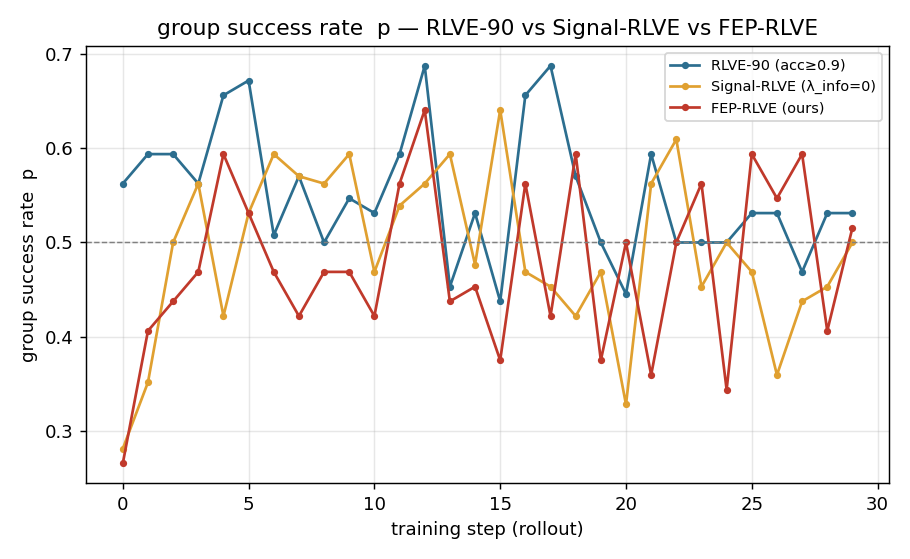
\includegraphics[width=0.48\linewidth]{figures/success_rate.png}\hfill
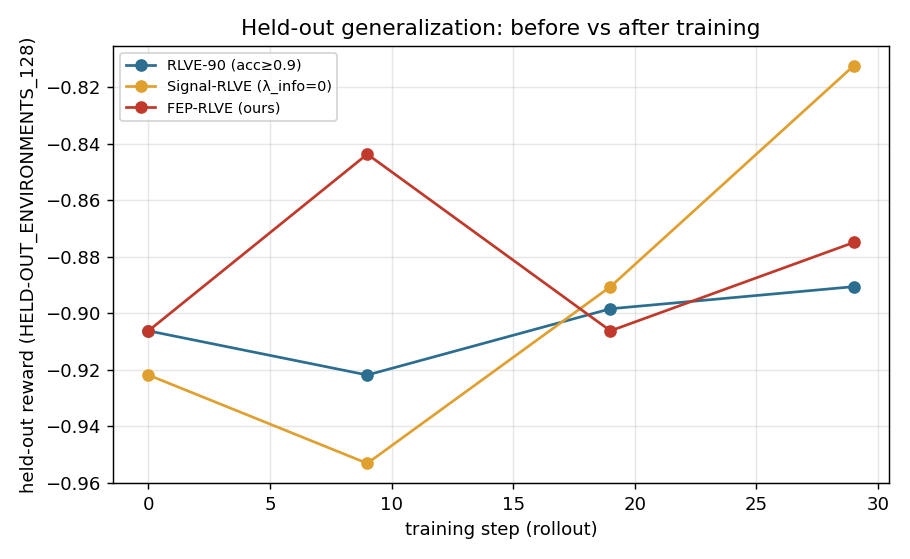
\includegraphics[width=0.48\linewidth]{figures/heldout.png}
\caption{\textbf{Left:} training group success vs.\ step; the EFE arms hold near
the $0.5$ set-point (dashed) while RLVE-90 sits higher. \textbf{Right:} held-out
reward before vs.\ after training---flat and near-floor for all arms; differences
are within noise.}
\label{fig:results}
\end{figure}

\paragraph{Mechanism: why the arms do not separate.}
Process diagnostics (Fig.~\ref{fig:diag}) tell a consistent story. (i) Response
\emph{truncation} is pinned at $0.7$--$0.9$ throughout training (and $\approx0.98$
at eval), so the model frequently hits the $2048$-token budget before emitting a
verifiable answer. (ii) With truncation $=$ failure, many $K{=}4$ groups become
\emph{degenerate} (all samples truncate/fail), so the realized advantage variance
collapses and the policy-gradient loss stays at $\sim\!2\times10^{-4}$---orders of
magnitude below a healthy run. (iii) Policy entropy nonetheless drops $\approx40\%$,
so the model commits without acquiring transferable skill, and held-out stays
floored. Crucially, training success $\approx0.5$ is therefore \emph{manufactured
by the controller selecting solvable difficulties}, not by the model improving:
a flat $0.5$ curve is evidence the controller works, not that capability rose.

\begin{figure}[t]
\centering
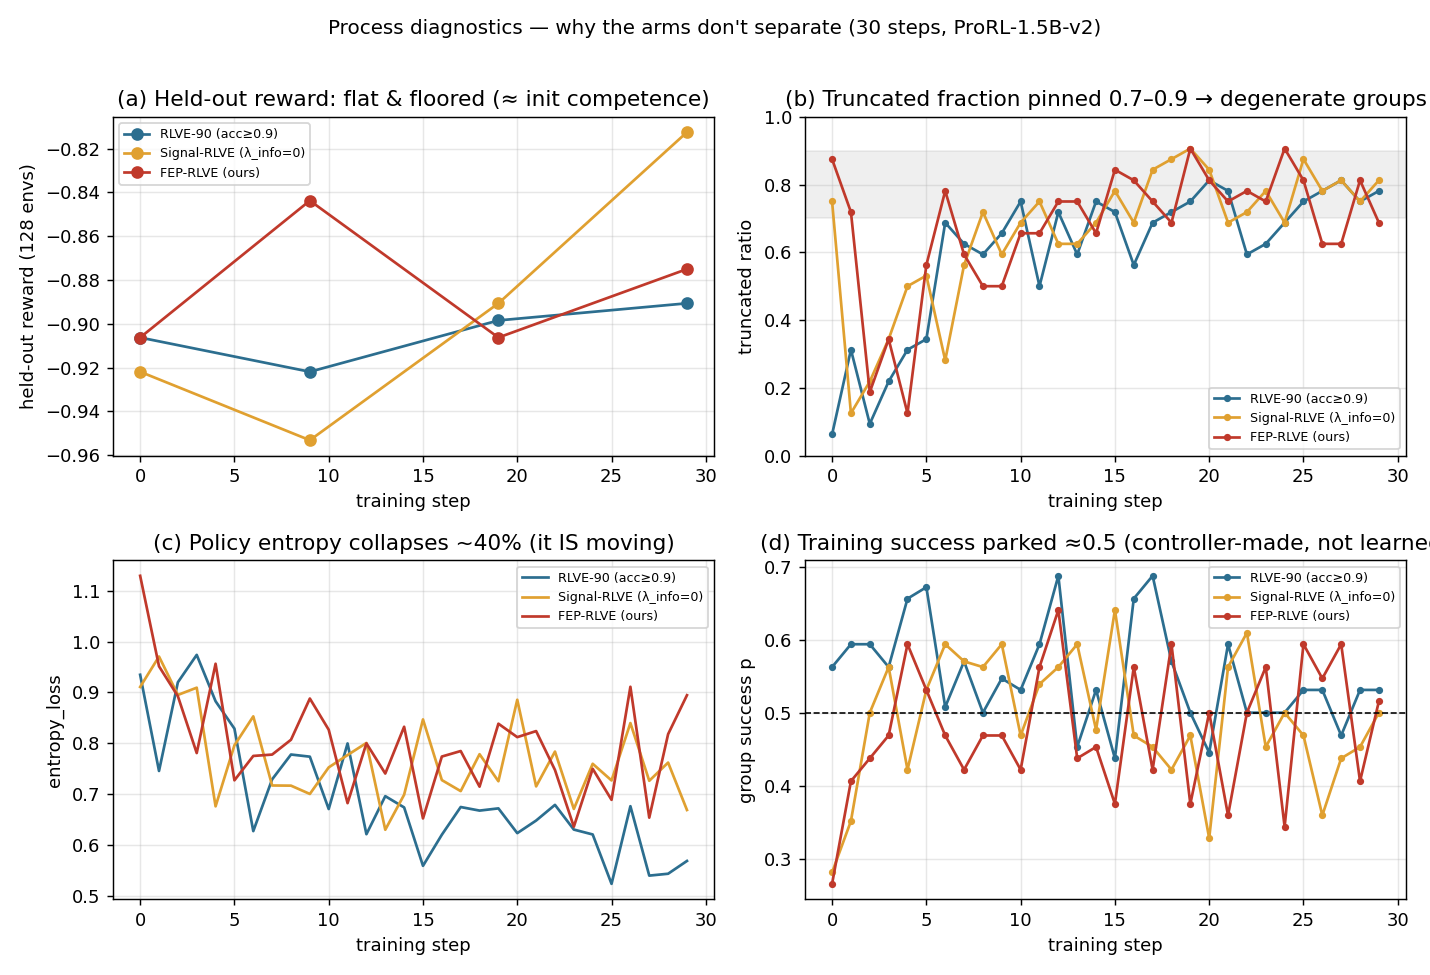
\includegraphics[width=0.92\linewidth]{figures/diagnostics.png}
\caption{Process diagnostics. (a) held-out is flat/floored for all arms; (b)
truncation pinned $0.7$--$0.9$; (c) policy entropy collapses $\approx40\%$; (d)
training success parked near $0.5$ (controller-made, not learned).}
\label{fig:diag}
\end{figure}

\section{Discussion and limitations}
\label{sec:discussion}
\textbf{Expected vs.\ realized signal.} $\UK(p)$ assumes the $K$ samples in a
group are \emph{independent} Bernoulli$(p)$ draws of correctness, giving
$\UK\approx0.85$ here. Truncation breaks this: when most completions are cut off,
group outcomes become correlated and degenerate, so the \emph{realized}
informative fraction is far below the \emph{expected} $\UK$. The effective-ratio
metric, computed from the same closed form, is blind to this degeneracy by
construction. This gap---not the choice of controller---is the binding constraint
at this scale, and it is the clearest target for future work (raise the response
budget; decouple ``truncated'' from ``wrong'' in the reward; feed the
\emph{measured} non-degenerate-group fraction back into the utility so the
controller optimizes realized rather than expected informativeness).
\textbf{What this study does and does not establish.} It validates that the EFE
controller regulates difficulty as designed, and that higher training success
(RLVE-90) does \emph{not} imply better generalization---the motivating claim that
accuracy is the wrong curriculum signal. It does \emph{not} establish a
generalization win for any arm: $30$ steps at $1.5$B with a floored, truncation-
suppressed held-out set leave no room for transfer to appear, and the held-out
gaps are within single-seed noise. \textbf{Other limitations.} Competence is
modeled as a single scalar $s_e$ per environment (real skills are
multi-dimensional and shared across environments); environments are modeled
independently, ignoring transfer. When the model outgrows $d_{\max}$ all levels
saturate ($\UK\!\to\!0$ everywhere) and \emph{no} controller has signal,
motivating environment scaling~\citep{zeng2025rlve,scaler2026}.

\section{Related work}
RL from verifiable rewards~\citep{lambert2024rlhf} and its environment-scaling
form RLVE~\citep{zeng2025rlve} and SCALER~\citep{scaler2026} regulate difficulty
toward the capability frontier; we replace their accuracy heuristic with an
explicit free-energy objective. Group-relative RL (GRPO~\citep{shao2024deepseekmath},
DAPO~\citep{yu2025dapo}) motivates the informative-group utility; ProRL~\citep{liu2025prorl}
is our base model. Our formulation is an instance of active inference / the Free
Energy Principle~\citep{friston2010free,dacosta2020active}, and the epistemic term
connects to learning-progress automated curricula~\citep{graves2017curriculum},
which it generalizes through an explicit belief over competence.

\section{Conclusion}
Casting difficulty selection as active inference replaces RLVE's accuracy-threshold
heuristic with a principled objective---a Bayesian belief over competence plus an
expected-free-energy criterion---that targets the signal-optimal operating point,
actively probes competence, and moves difficulty both ways, at near-zero extra
compute and with the RL core unchanged. In a small-scale reproduction the
controller regulates difficulty as designed; honest diagnostics show that
response truncation, not the controller, currently caps learning by collapsing the
realized gradient below the expected one. Closing that expected-vs-realized gap is
the natural next step.

\bibliographystyle{plainnat}
\bibliography{refs}

\appendix
\section{Why the learning signal is maximized at \texorpdfstring{$p=0.5$}{p=0.5}}
\textbf{A.1 Vanishing advantages on zero-variance groups.} GRPO/DAPO set
$A_j=(r_j-\bar r)/(\sigma_r+\varepsilon)$ with $\bar r=k/G$ and
$\sigma_r^2=\hat p(1-\hat p)$ for $k$ correct of $G$. If $k\in\{0,G\}$ then
$\sigma_r=0$ and all $A_j=0$: no gradient. \textbf{A.2 Informative-group
probability.} $P_{\mathrm{inf}}(p)=1-(1-p)^G-p^G$; $P_{\mathrm{inf}}'(p)=G[(1-p)^{G-1}-p^{G-1}]=0\Rightarrow p^\star=1/2$,
a maximum for all $G\ge2$. \textbf{A.3 Variance.} $\mathrm{Var}[r]=p(1-p)$ peaks at
$0.5$ and the expected empirical variance $p(1-p)(1-1/G)$ shares the maximizer, so
both the \emph{frequency} of informative groups and the \emph{magnitude} of their
advantages peak at $p=0.5$. \textbf{A.4 Consequence.} Since $p(d)$ is decreasing
in $d$, some $d^\star$ gives $p=0.5$; RLVE's $\tau_{\mathrm{acc}}{=}0.9$ keeps the
model at low $\UK$ and never lowers difficulty. For shaped rewards the optimum
shifts off $0.5$ to wherever $\mathrm{Var}[r]$ is maximal and $p^\star$ becomes a
tunable target.

\section{Active-inference formulation}
This is Friston's Free Energy Principle, not a thermodynamic energy$-$entropy
objective. \textbf{B.1 Generative model:} $P(o{=}1\mid s_e,d)=\sigma(a(s_e-d))$,
belief $q(s_e)$, $\hat p(d)=\mathbb{E}_{s\sim q}[\sigma(a(s-d))]$. \textbf{B.2
Perception:} minimizing $F[q]=\KL(q(s)\|p(s\mid o))-\ln p(o)$ gives the exact grid
posterior $q(s)\leftarrow q(s)\prod_k P(o_k\mid s,d_k)/Z$. \textbf{B.3 Pragmatic
term:} preferring informative outcomes gives risk $-\ln \UK(\hat p)$, which
diverges as $\UK\!\to\!0$. \textbf{B.4 Epistemic term:}
$I_q(s_e;o\mid d)=H[\mathrm{Ber}(\hat p)]-\mathbb{E}_{s\sim q}H[\mathrm{Ber}(\sigma(a(s-d)))]$.
\textbf{B.5 Policy:} $\pi(d\mid e)\propto\exp(-G_e(d)/T)$; RLVE is
$\lambda_{\mathrm{info}}{=}0$, $T\!\to\!0$, high-accuracy preference.

\section{Reproduction}
Single-GPU RLVE reproduction steps and the controller integration point are in
\texttt{rlve\_repro/} (\texttt{active\_inference\_controller.py},
\texttt{active\_inference\_manager.py}); analysis and figures are regenerated by
\texttt{analyze\_rlve.py} and \texttt{diagnostics.py}.

\end{document}
